\chapter{Overview of existing methods}
\addtocontents{toc}{\contentsline{chapter}{Methods}{\protect\pageref{annotation}}}
\label{ch:Methods}

This chapter presents some of the well-established methods of approximating the wavefunctions of multi-electron atoms. The Thomas-Fermi model that eventually led to the development of Density Functional Theory, the Hartree-Fock method that forms the basis of many modern high-precision atomic calculation schemes and the perturbation series in the inverse of the nuclear charge.

\section{The Thomas-Fermi model}
\label{sec:TF}

The main idea of the TF model is to look for the form of electron density, as a function of space $n(\vec{r})$, rather than the multi-electron wavefunction, as a function of the positions of individual electrons: $\Psi(\vec{r_1} ... \vec{r_N})$. This is done by writing the total energy of the electron cloud as a functional of the electron density, and looking for its minimum: 
\begin{equation}
     E[n(\vec{r})] = E_{kin}[n(\vec{r})] + U_{eN}[n(\vec{r})] + U_{ee}[n(\vec{r})],
\end{equation}
where $U_{eN}$ and $U_{ee}$ are the electron-nucleus and electron-electron potential energies respectively.

Assuming that electrons are uniformly distributed in phase space up to the Fermi momentum, with the classical expression for kinetic energy $E_{kin} = p^2/2$, one can obtain the density functional as~\cite{lundqvist2013theory}: 
\begin{equation} \label{TFenergy}
     E[n(\vec{r})] = C_{\rm{kin}}\int n(\vec{r})^{5/3} d \vec{r} + \int V_{N}(\vec{r})n(\vec{r}) d \vec{r} + \frac{1}{2} \int \frac{n(\vec{r_1}) n(\vec{r_2})}{|\vecr{r_1}-\vec{r_2}|} d\vec{r} d\vec{r_2},
\end{equation}
where $V_N$ is the nuclear potential and $C_{\rm{kin}}$ is a numerical constant related to the volume of occupied phase space, in this case: $C_{\rm{kin}} \approx 2.8712$.

The task is then to minimize the energy, while keeping the number of electrons $N$ constant:
\begin{equation}
    \int n(\vec{r})d \vec{r} = N.
\end{equation}

This can be achieved using a Lagrange multiplier $\mu$, called chemical potential, given by:
\begin{align}
\mu = \frac{5}{3} C_{kin} n(\vec{r})^{2/3} + V(\vec{r}),
\end{align}
where $V$ is the total (effective) potential:
\begin{align}
V(\vec{r}) = V_{N}(\vec{r}) + \int \frac{n(\vec{r_2})}{|\vec{r_2}-\vec{r}|} d\vec{r_2},
\end{align}
and looking for the form of $V(\vec{r})$ that corresponds to a stationary point. The numerical value of $\mu$ is related to the difference between the nuclear charge and the number of electrons, so that $\mu = 0$ for neutral atoms and $\mu < 0$ for positive ions.

In the case of a spherically symmetric nucleus, the total potential becomes a one-dimensional function $V(\vec{r}) = V(r)$. For the case of a point-like nucleus $V_N = -\frac{Z}{r}$, the effective potential can be expressed as:
\begin{align}
V(r) = \mu - \frac{Z}{r} \phi \left(\frac{r}{b}\right),~~~~~~~~~~b=\frac{1}{4}\left(\frac{9\pi^2}{2Z}\right)^{1/3}.
\end{align}
The potential $V(r)$ is then a stationary point of \eqref{TFenergy} whenever the function $\phi(r)$ satisfies the so-called Thomas-Fermi equation~\cite{davis1962introduction}:
\begin{equation} \label{TFequation}
    \frac{\partial^2 \phi(r)}{\partial r^2} = \frac{\phi^{3/2}(r)}{\sqrt{r}},
\end{equation}
with boundary conditions $\phi(0)=1$ and $\phi(+\infty)=0$.

This deceptively simple looking differential equation has no analytical solution and is plagued by a somewhat famous numerical problem. In order to propagate a numerical solution of \eqref{TFequation} from the origin, it is necessary to know the initial slope $\phi'(0)$, which cannot be calculated analytically. Furthermore, even slight deviation from its critical value can lead to an entirely wrong behaviour. If the value of the initial slope is bigger than the critical value, the numerically propagated $\phi(r)$ diverges at a finite $r$ and if it's smaller, it crosses the real line whereby becoming complex (see figure~\ref{TFfig}). An algorithm for calculating the critical value of $\phi'(0)$ was first developed by Ettore Majorana in 1928~\cite{1.1484144}, and considerable effort has since gone into improving it, including in recent years~\cite{LIU2015251,PARAND2017624,pub1041457795}.
\begin{figure} [t] 
	\centering
	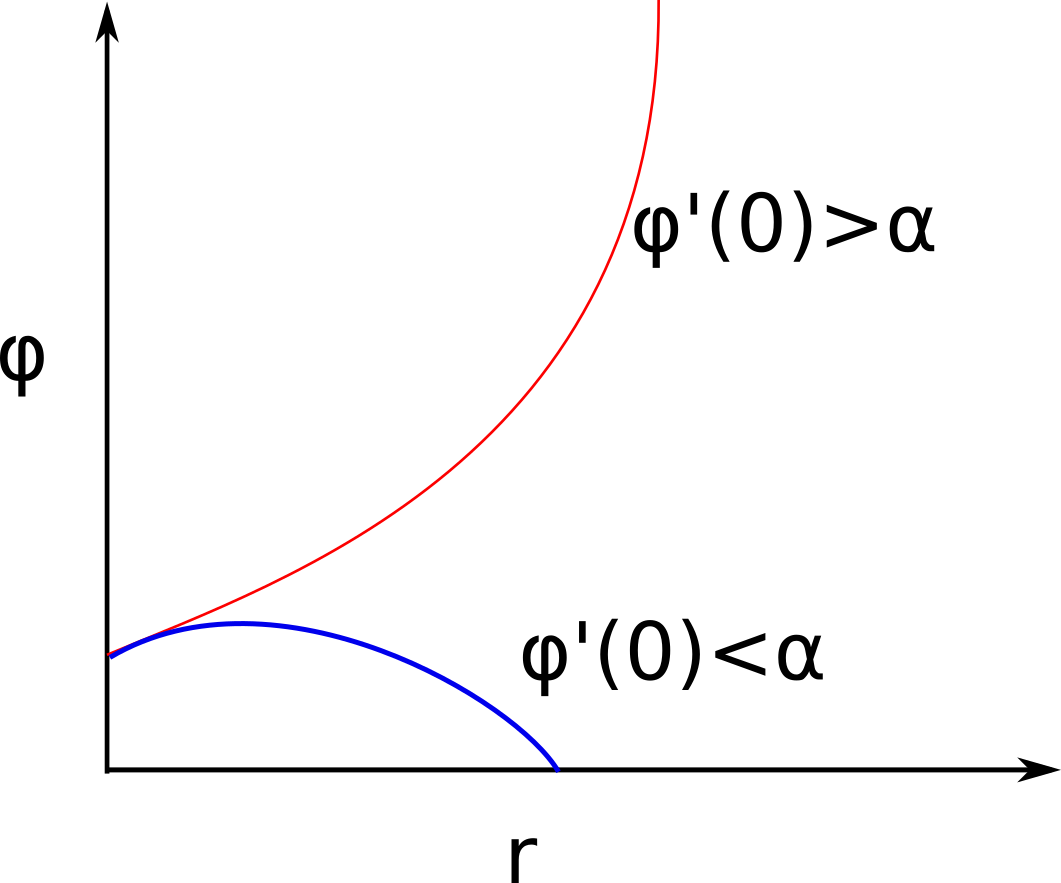
\includegraphics[width=80mm]{Graphs/TF.png} 
	\caption{Pictorial representation of the numerical difficulties associated with finding normalizable solutions of the Thomas-Fermi equation. The initial value $\phi(0)$ is given, but the initial slope $\phi'(0)$ needs to be found by trial and error. If the value is higher that the critical value $\alpha$, the numerically propagated solution diverges. If it is lower, the solution hits the real line and becomes complex.} \label{TFfig}
\end{figure}

\section{The Hartree-Fock method}

The main idea of the HF method is to look for a distribution of electrons self-consistent with a field that it generates. The first step is to specify the ground state configuration, that is, a set of occupied electron orbitals $\phi_i$. Then an initial approximation to the shape of all of those occupied single-electron orbitals is needed. This can be done using the Thomas Fermi model, or by solving the corresponding problem without the electron-electron interaction.
In order to ensure anti-symmetry, the total multi-electron wavefunction is represented by a Slater determinant of single-electron orbitals:
\begin{equation} \label{HFdet}
  \Phi(\vec{r_1}, \vec{r_2} ... \vec{r_N}) = \frac{1}{\sqrt{N!}}
   \left| \begin{matrix} \phi_1(\vec{r_1}) & \phi_2(\vec{r_1}) & \dots & \phi_2(\vec{r_1}) \\
    \vdots & & \ddots &  \\ 
    \phi_1(\vec{r_N}) & \phi_2(\vec{r_N})& \dots & \phi_N(\vec{r_N})  \end{matrix} \right|.
\end{equation}

The influence of electron-electron interaction is then taken into account using the mean-field approximation, meaning that any given electron is assumed to occupy a bound state in the potential formed by all of the other electrons and the nucleus. This means that for the $i^{\rm{th}}$ electron we can find the so-called Fock operator $\widehat{F}_i$ given by~\cite{560430312}:
\begin{equation}
    \widehat{F}_i = \widehat{H}_i+\sum_j^n (\widehat{J}_{ij} - \widehat{K}_{ij}),
\end{equation}
where $\widehat{J}_{ij}$ and $\widehat{K}_{ij}$ are the Coulomb and exchange operators describing the interaction between the $i^{\rm{th}}$ and $j^{\rm{th}}$ electrons, and $\widehat{H}_i$ is the single particle Hamiltonian of the $i$ electron, including it's kinetic energy and interaction with the nucleus. If the relativistic version of $H_i$ is used, then the method is referred to as Dirac-Hartree-Fock (DHF) procedure.

Each of the Fock operators can then be diagonalized:
\begin{equation}
    \widehat{F}_i \phi_i = E_i \phi_i,
\end{equation}
to obtain a new set of occupied orbitals $\phi_i$. This process is repeated until a specified level of accuracy is reached. The schematic representation of this algorithm is presented in figure~\ref{HFalgo}.

When implementing the HF procedure in a computer program, in order to efficiently diagonalize the set of Fock operators $\widehat{F}_i$, the occupied orbitals $\phi_i$ are typically expanded in a basis, that allows for rapid evaluation of Coulomb and exchange integrals. This means that the whole computation is reduced to the repeated calculation of the expansion coefficients of the orbitals. Popular choices of basis sets include Gaussian functions, B-splines,~\cite{FROESEFISCHER20111315} and Sturmian functions~\cite{sturmian}.

The variational principle~\cite{epstein2012variation} tells us, that the expectation value of the Hamiltonian with any wavefunction is higher than the ground state energy, which means that the Hartree-Fock procedure always provides an upper bound on the ground state energy (this is not necessarily the case for excited states~\cite{LandauQM}).

\begin{figure} [t] 
	\centering
	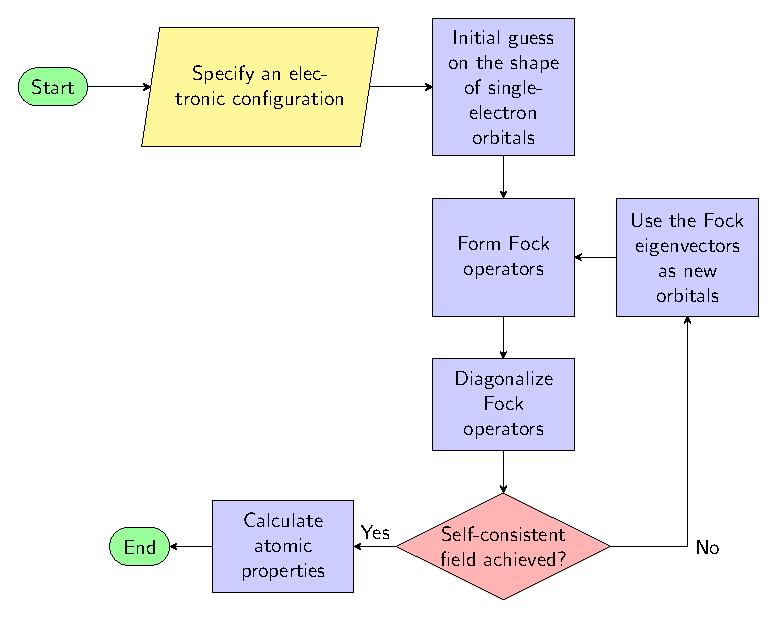
\includegraphics[width=119mm]{Graphs/HFalgorithm.pdf} 
	\caption{Pictorial representation of the basic algorithm behind using the HF method to calculate properties of multi-electron atoms.} \label{HFalgo}
\end{figure}

Because of the mean-field approximation described above, all electron-electron correlation beyond the anti-symmetry relation is neglected. This is typically the main source of uncertainty in the Hartree-Fock procedure. Numerous approaches have since been developed to incorporate the effects of correlation, collectively know as post-Hartree-Fock methods. One of the most straightforward methods is the configuration interaction (CI)~\cite{Tup2003OS}. It replaces the single Slater determinant with a more general representation of a linear combination of multiple Slater determinants (often also referred to as configurations):
\begin{equation}
  \Psi(\vec{r_1}, \vec{r_2} ... \vec{r_N}) = \sum_I c_I \Phi_I(\vec{r_1}, \vec{r_2} ... \vec{r_N}),
\end{equation}
where $\Phi_0$ is given by \eqref{HFdet}, and the remaining $\Phi_I$ are formed by replacing some number of the occupied orbitals by virtual orbitals. In order to save computational time, the CI-space must be truncated, meaning that only determinants that differ from $\Phi_0$ up to a certain number of orbitals are used. In general, the use of multiple configurations, or other post-Hartree Fock methods, can greatly increase accuracy, but also requires significantly larger computational time~\cite{Koppl2016}.

\section{Perturbation theory of multi-electron atoms}

The general setup of a perturbative calculation is to write the total Hamiltonian $H$ as a sum of the solvable unperturbed operator $H^0$ and a perturbation operator $W$:
\begin{equation}
	\widehat{H}=\widehat{H}^0+\lambda \widehat{W},
\end{equation}
where $\lambda$ is a parameter characterising the strength of the perturbation. The solution of the unperturbed problem is written as: 
\begin{equation}
	\widehat{H}^0|\psi^0_n\rangle=E^0_n|\psi^0_n\rangle.
\end{equation}

Now, since the eigenvectors of a Hermitian operator form an orthonormal basis $\langle \psi^0_n|\psi^0_k\rangle = \delta_{kn}$, we can expand the full problem in that basis, i.e. write the full energy as a power series in $\lambda$. The first two corrections read~\cite{19263840404}: 
\begin{align} \label{PertSeries}
	E_n(\lambda) =& E^{(0)}_n + \lambda \Delta E^{(1)}_n + \lambda^2 \Delta E^{(2)}_n + O[\lambda^3] \nonumber \\
	 =& \langle \psi_n^0 |\widehat{H}^0|\psi_n^0\rangle + \lambda \langle \psi^0_n|\widehat{W}|\psi^0_n\rangle+\lambda^2 \sum_{k \neq n} \frac{|\langle \psi^0_n|\widehat{W}|\psi^0_k\rangle|^2}{E^0_n-E^0_k} + O[\lambda^3].
\end{align}
Similarly we can write the expansion of the eigenvectors as:
\begin{equation}
	|\psi_n\rangle (\lambda) = |\psi^0_n\rangle + \lambda  \sum_{k \neq n} \frac{\langle \psi^0_k|\widehat{W}|\psi^0_n\rangle}{E^0_n-E^0_k} |\psi^0_k\rangle + O[\lambda^2].
\end{equation}

In the particular case of multi-electron atoms, one traditionally takes the hydrogen Hamiltonian as the unperturbed problem, and the electron-electron interaction as the perturbation:
\begin{equation}
	\widehat{H}_0 = \sum_i \widehat{H}^{\rm{kin}}_i + \frac{Z}{r_i},~~~~~~~~~~\widehat{W} = \sum_{i<j} \frac{1}{|r_i-r_j|},
\end{equation}
where the single-electron kinetic part $\widehat{H}^{\rm{kin}}_i$ can be given by either Schr\"odinger or Dirac theories. This somewhat obvious choice leads to the so-called $1/Z$ expansion, as subsequent corrections are proportional to the decreasing powers of $Z$.


